\documentclass{article}
\usepackage{times}
\usepackage{amsmath, amssymb}
\usepackage{graphicx}
\usepackage{algorithm}
\usepackage{algorithmic}
\usepackage{hyperref}
\usepackage{booktabs}

\title{Local Spectral Retrieval: Variance-Aware Neighbor Selection via PCA in Thresholded Embedding Neighborhoods}

\author{
  Alison Cossette \\
  \texttt{alison@claritrace.com}
}

\begin{document}

\maketitle

\begin{abstract}
This paper introduces \textbf{Local Spectral Retrieval (LSR)}, a retrieval method that improves embedding-based search by incorporating the local geometric structure of threshold-defined neighborhoods. Traditional cosine-based retrieval treats each neighbor independently and is insensitive to redundancy caused by density collapse. LSR first performs radius-based retrieval using a minimum cosine similarity threshold, then applies Principal Component Analysis to the resulting neighborhood. It then samples $k$ neighbors that maximize variance along the dominant principal direction, producing a diverse, non-redundant set of documents. Experiments on multiple QA benchmarks demonstrate that LSR improves multi-hop recall, reduces redundancy, and enhances RAG answer accuracy. 
\end{abstract}


\section{Introduction}

Embedding-based retrieval sits at the core of modern information access systems, including vector databases, large language model (LLM) retrieval-augmented generation (RAG), and search pipelines built on dense neural representations. The dominant approach---ranking documents by cosine similarity and selecting the top-$k$---assumes that local neighborhoods in embedding space are well-behaved, smoothly distributed, and structurally informative. In practice, however, this assumption rarely holds. Real-world corpora contain paraphrase clusters, boilerplate text, templated content, and highly redundant segments, all of which can collapse into dense regions of embedding space. As a result, cosine similarity often retrieves many near-duplicate neighbors, hurting diversity, factual coverage, and downstream reasoning performance.
\par
Threshold-based retrieval methods, such as radius or similarity cutoff queries supported by vector databases, attempt to improve recall by returning all points above a minimum similarity level. While effective in theory, these methods amplify the redundancy problem: dense semantic regions may contain dozens or hundreds of highly similar vectors that all satisfy the threshold, overwhelming top-$k$ selection and producing context that is unnecessarily repetitive. This behavior is especially problematic in multi-hop or compositional question answering, where retrieving diverse pieces of evidence is more important than retrieving multiple versions of the same fact.
\par
Dense retrieval systems\cite{karpukhin2020dense} and modern vector databases such as FAISS\cite{johnson2019billion} form the backbone of RAG pipelines \cite{lewis2020rag}.
\par
A key limitation of cosine similarity---and of most existing retrieval strategies built on it---is that it is \emph{pointwise}. The similarity between a query and each candidate is evaluated independently, without regard for the geometric structure of the neighborhood itself. Important local properties such as variance, redundancy structure, and principal directions of semantic change are ignored. In dense regions, the local covariance is often dominated by one or two principal components, revealing that the neighborhood collapses along a low-dimensional manifold. Cosine similarity cannot detect this collapse, nor can it use spectral information to diversify selection.
\par
This paper introduces \textbf{Local Spectral Retrieval (LSR)}, a simple but effective method that incorporates local geometric structure into the retrieval process. LSR first performs threshold-based retrieval to form a high-recall semantic neighborhood, then applies Principal Component Analysis (PCA) to characterize the neighborhood's internal structure. Finally, LSR selects $k$ neighbors by sampling along the dominant principal direction, ensuring that the returned set spans the local variance instead of collapsing onto redundant points. This approach preserves the strengths of threshold-based retrieval while mitigating its tendency to surface repetitive or low-information neighbors.

The contributions are threefold:
\begin{enumerate}
    \item Identification and formalization of the issue of \emph{density collapse} in high-dimensional embedding retrieval, showing how threshold-based methods exacerbate redundancy.
    \item A retrieval framework, LSR, that leverages local PCA to select a variance-maximizing subset of neighbors from the threshold-defined region.
    \item Empirical demonstration that LSR improves evidence diversity, multi-hop recall, and RAG answer quality across several QA benchmarks, while adding minimal computational overhead.
\end{enumerate}

LSR offers a practical, interpretable, and geometry-aware alternative to traditional top-$k$ and MMR-based retrieval, advancing toward retrieval methods that better reflect the manifold structure of modern embedding spaces.

\section{Related Work}

\subsection{Cosine Similarity and Top-$k$ Retrieval}
Dense embedding retrieval systems typically rely on cosine similarity or dot-product scoring to identify relevant neighbors \cite{johnson2019billion, karpukhin2020dense}. The dominant paradigm selects the top-$k$ highest-scoring vectors for downstream use. While effective for identifying individually relevant items, top-$k$ retrieval is inherently pointwise: it evaluates each candidate independently with no awareness of the structure or redundancy within the retrieved set. This often results in multiple near-duplicate neighbors in dense regions of embedding space, reducing contextual diversity and limiting downstream reasoning performance.

\subsection{Threshold and Radius-Based Retrieval}
Modern vector databases such as FAISS\cite{johnson2019billion}, Milvus, and OpenSearch support similarity-threshold or radius queries, which return all points within a specified distance or similarity cutoff. Such methods improve recall and allow adaptive neighborhood sizes, but they also exacerbate redundancy when large clusters of nearly identical vectors satisfy the threshold. Prior work on high-dimensional search structures, including HNSW \cite{malkov2018efficient} and IVF-based quantization methods \cite{jegou2011product}, focuses primarily on approximate search efficiency rather than improving the semantic quality or diversity of retrieved neighbors. To our knowledge, no prior method systematically analyzes or mitigates density collapse within threshold-defined neighborhoods.
Radius-based search is supported by modern ANN systems including FAISS \cite{johnson2019billion}, Milvus, and HNSW-based methods \cite{malkov2018efficient}.

\subsection{Diversified Retrieval and Re-ranking}
To counter redundancy in top-$k$ retrieval, several diversification techniques have been proposed. Maximal Marginal Relevance (MMR) \cite{carbonell1998mmr} and more recent neural variants \cite{ray2023learning} aim to balance relevance and novelty by penalizing similarity to previously selected items. Other approaches leverage submodular optimization \cite{lin2012learning}, clustering-based selection \cite{xia2022dense}, or coverage-based scoring to improve diversity. While effective, these methods operate on pairwise similarities among candidates and do not incorporate geometric information such as principal directions or eigenvalue structure. As a result, they remain less sensitive to low-dimensional collapse within high-density regions.

\subsection{PCA and Spectral Methods in Retrieval}
Principal Component Analysis and related spectral methods have been widely used for dimensionality reduction, clustering, and indexing. PCA-trees \cite{sproull1991pca} and spectral partitioning methods exploit principal directions to construct efficient search structures, but these techniques focus on global or recursive partitioning and do not use PCA to analyze local neighborhoods returned by similarity search. More recent work on dimensionality-reduced retrieval for RAG \cite{park2024pca} applies PCA to embeddings globally, typically for compression or efficiency, not for diversity-aware neighbor selection. In contrast, LSR performs \emph{local} PCA on the threshold-defined region, using spectral variance directly to guide neighbor selection.

\subsection{Retrieval-Augmented Generation}
RAG systems rely heavily on the quality and diversity of retrieved evidence \cite{lewis2020rag, izacard2021leveraging}. Prior studies show that redundancy in retrieved documents reduces faithfulness, increases hallucinations, and degrades multi-hop performance. Approaches to improve RAG often focus on re-ranking, query reformulation, or iterative retrieval \cite{khattab2021relevance, trivedi2022contextual}. For multi-hop reasoning specifically, GraphRAG \cite{edge2024graphrag} constructs knowledge graphs over documents and traverses them to gather evidence from structurally connected but semantically distinct sources---an effective approach when explicit entity relationships are available. However, few works examine the geometric structure of embedding neighborhoods themselves. LSR is complementary to graph-based approaches: it operates directly on the embedding space without requiring graph construction, making it applicable as a lightweight post-retrieval filter in any vector-search pipeline, including those that feed into graph-based reasoning stages.

\subsection{Summary}
Across top-$k$ retrieval, threshold search, diversification strategies, and spectral methods, prior work has not fully addressed the challenge of density collapse in local embedding neighborhoods. This work addresses this gap by introducing a geometry-aware retrieval strategy that leverages local PCA structure to guide variance-maximizing neighbor selection.

\begin{figure}[t]
    \centering
    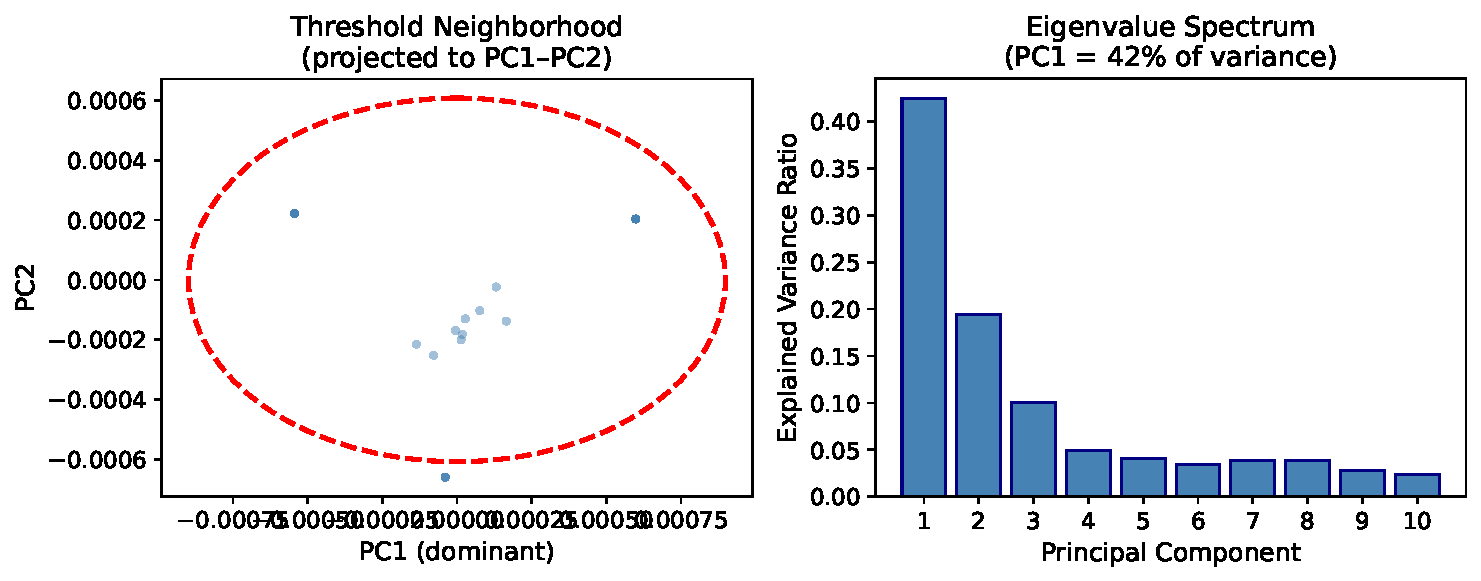
\includegraphics[width=0.75\linewidth]{figs/density_collapse.pdf}
    \caption{
        Example of density collapse in a threshold-defined neighborhood.
        Although the neighborhood contains many points above the similarity threshold,
        most lie along a low-dimensional manifold. Cosine similarity alone cannot detect
        this redundancy, motivating the need for variance-aware selection.
    }
    \label{fig:density-collapse}
\end{figure}

\section{Problem Formulation}

Let $\{x_i\}_{i=1}^N$ denote a corpus of embedding vectors in $\mathbb{R}^d$, and let $q \in \mathbb{R}^d$ be the query embedding. Retrieval systems typically identify relevant items by computing the cosine similarity
\begin{equation}
    s(q, x_i) = \frac{q^\top x_i}{\|q\|\|x_i\|},
\end{equation}
and selecting either the top-$k$ highest-scoring vectors or all vectors whose similarity exceeds a threshold $\tau$.

\subsection{Threshold-Based Neighborhoods}
In threshold retrieval, the system returns the set:
\begin{equation}
    \mathcal{N}(q, \tau) = \{ x_i : s(q, x_i) \ge \tau \}.
\end{equation}
This region forms a high-recall neighborhood around the query. However, when the embedding distribution contains dense clusters or low-variance manifolds, $\mathcal{N}$ may contain many redundancies. In practice, $|\mathcal{N}|$ can range from a handful of items to hundreds, depending on corpus density and the value of $\tau$.
Modern vector search systems such as FAISS \cite{johnson2019billion} and HNSW-based engines \cite{malkov2018efficient} support radius and similarity-threshold queries.

The goal is to select a subset $\mathcal{S} \subseteq \mathcal{N}$ of size $k$ that is both relevant and diverse. Formally, the objective is to preserve semantic compatibility with the query while maximizing coverage of the local geometric structure of $\mathcal{N}$.

\subsection{Density Collapse in Embedding Space}
Empirically, threshold neighborhoods often exhibit \emph{density collapse}: most of the variance is concentrated along one or two directions. Let $\mu$ denote the mean of $\mathcal{N}$ and let the centered matrix be
\begin{equation}
    Z = [x - \mu : x \in \mathcal{N}]^\top.
\end{equation}

The local covariance matrix is
\begin{equation}
    C = \frac{1}{|\mathcal{N}|} Z^\top Z.
\end{equation}

The eigenvalues $\lambda_1 \ge \lambda_2 \ge \cdots \ge \lambda_d$ characterize the variance distribution within the neighborhood. In dense regions, it is common to observe a strongly dominant first component,
\begin{equation}
    \lambda_1 \gg \lambda_2, \lambda_3, \ldots,
\end{equation}
indicating that most variation lies along a single direction. This collapse leads to redundancy: many points in $\mathcal{N}$ are near-duplicates or paraphrases, differing only slightly along the dominant axis. Cosine similarity alone cannot detect this structure, as it treats each point independently.

\subsection{Objective: Variance-Aware Selection}
Given a threshold-defined neighborhood $\mathcal{N}$ with covariance eigenstructure $(\lambda_j, v_j)$, this work defines a selection function
\begin{equation}
    \text{Select}_k : \mathcal{N} \rightarrow \mathcal{S} \subseteq \mathcal{N},
\end{equation}
such that:
\begin{enumerate}
    \item $\mathcal{S}$ contains $k$ items relevant to the query, and
    \item $\mathcal{S}$ spans a maximal portion of the local variance of $\mathcal{N}$.
\end{enumerate}

For practical retrieval systems, the selection should satisfy additional constraints:
\begin{itemize}
    \item \textbf{Low additional cost:} The method must be lightweight compared to similarity search.
    \item \textbf{Locality:} Computation depends only on $\mathcal{N}$, not on the global corpus.
    \item \textbf{Interpretability:} The mechanism should provide insight into neighborhood structure.
\end{itemize}

\subsection{Local Spectral Retrieval}
Local Spectral Retrieval (LSR) instantiates the selection problem by projecting all points in $\mathcal{N}$ onto the leading principal component $v_1$ and sampling points that best cover the induced one-dimensional structure. Operating on the spectral geometry of the neighborhood rather than pointwise similarities, LSR directly addresses the collapse phenomenon and promotes meaningful diversity in the retrieved set.

\section{Local Spectral Retrieval (LSR)}

\begin{algorithm}[h]
\caption{Local Spectral Retrieval (LSR)}
\begin{algorithmic}
\STATE \textbf{Input:} query $q$, dataset $X$, threshold $\tau$, sample size $k$
\STATE $\mathcal{N} \leftarrow \{ x \in X : \cos(q,x) \geq \tau \}$
\IF{$|\mathcal{N}| \leq k$}
  \RETURN $\mathcal{N}$
\ENDIF
\STATE compute $\mu$ and covariance $C$
\STATE compute top eigenvector $v_1$ and eigenvalues $\lambda_1, \ldots, \lambda_d$
\FOR{$x \in \mathcal{N}$}
  \STATE $p(x) \leftarrow v_1^\top (x - \mu)$
\ENDFOR
\STATE sort $\mathcal{N}$ by $p(x)$
\STATE select $k$ points by quantile sampling
\RETURN selected $k$ points
\end{algorithmic}
\end{algorithm}

\begin{algorithm}[h]
\caption{Adaptive LSR}
\begin{algorithmic}
\STATE \textbf{Input:} query $q$, dataset $X$, threshold $\tau$, sample size $k$
\STATE $\mathcal{N} \leftarrow \{ x \in X : \cos(q,x) \geq \tau \}$
\IF{$|\mathcal{N}| \leq k$}
  \RETURN $\mathcal{N}$
\ENDIF
\STATE compute PCA on $\mathcal{N}$; obtain $r_1 = \lambda_1 / \sum_j \lambda_j$
\IF{$r_1 \geq 0.70$}
  \STATE \textit{// Strong collapse: standard LSR}
  \RETURN quantile sample along $v_1$
\ELSIF{$r_1 \geq 0.50$}
  \STATE \textit{// Moderate collapse: two-component LSR}
  \RETURN grid sample along $v_1, v_2$
\ELSE
  \STATE \textit{// Weak collapse: fallback}
  \RETURN MMR or top-$k$ selection
\ENDIF
\end{algorithmic}
\end{algorithm}

Local Spectral Retrieval (LSR) aims to improve the diversity and informativeness of retrieved neighbors by leveraging the spectral structure of threshold-defined embedding neighborhoods. Rather than selecting the top-$k$ points by cosine similarity or re-ranking candidates using pairwise penalties, LSR analyzes the local covariance geometry and selects documents that span the dominant directions of variance. This section details the method.

\subsection{Step 1: Constructing the Threshold Neighborhood}

Given a query embedding $q$, LSR begins by constructing the high-recall neighborhood
\begin{equation}
    \mathcal{N} = \{ x_i \in X : s(q, x_i) \geq \tau \},
\end{equation}
where $\tau$ is a similarity threshold. This operation is supported by most vector databases and efficiently executed using approximate nearest neighbor (ANN) indexes. Threshold retrieval typically yields a set whose size $|\mathcal{N}|$ varies with corpus density and query specificity.

If $|\mathcal{N}| \le k$, LSR simply returns all retrieved items. Otherwise, the method proceeds to variance analysis.

\subsection{Step 2: Local PCA on the Retrieved Neighborhood}
PCA-based neighborhood analysis has long been used to characterize local manifold structure \cite{sproull1991pca}.
To characterize the internal geometry of $\mathcal{N}$, LSR computes its mean
\begin{equation}
    \mu = \frac{1}{|\mathcal{N}|} \sum_{x \in \mathcal{N}} x
\end{equation}
and covariance
\begin{equation}
    C = \frac{1}{|\mathcal{N}|} \sum_{x \in \mathcal{N}} (x - \mu)(x - \mu)^\top.
\end{equation}

The leading eigenvector $v_1$ of $C$ is then computed, corresponding to the principal direction of maximum variance. In practice, computing only the top eigenpair is sufficient, and efficient power iteration makes this step inexpensive even for high-dimensional embeddings.

A key observation is that density collapse manifests as a dominant $\lambda_1$; thus, selecting points that spread along $v_1$ captures the essential variability of the region.

\subsection{Step 3: Projection onto the Dominant Direction}

Each point $x \in \mathcal{N}$ is projected onto the principal direction $v_1$:
\begin{equation}
    p(x) = v_1^\top (x - \mu).
\end{equation}

This transforms the high-dimensional neighborhood into a one-dimensional coordinate system aligned with its maximal variance. The distribution of the projected values $\{p(x)\}$ reflects how points spread or cluster along this direction, revealing local redundancy patterns.

\begin{figure}[t]
    \centering
    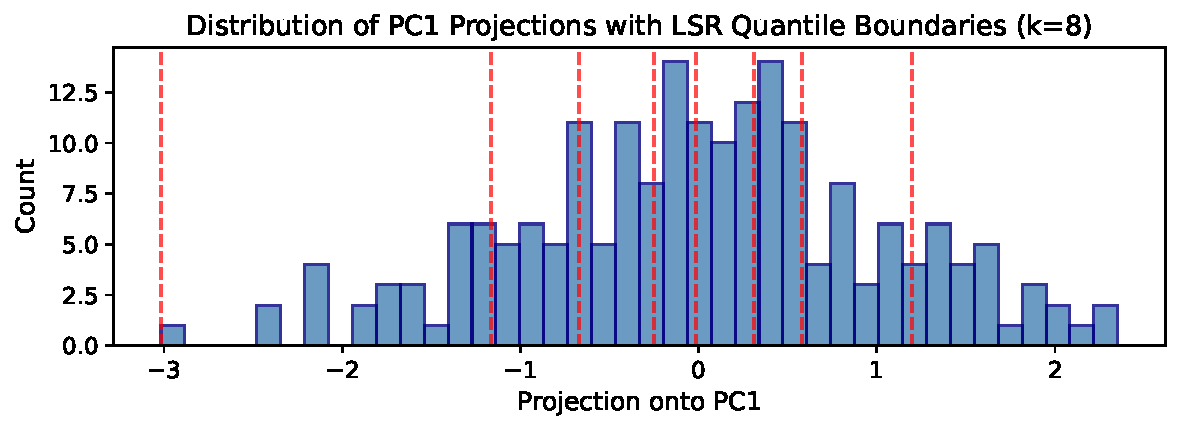
\includegraphics[width=0.75\linewidth]{figs/pc1_projection.pdf}
    \caption{
        Distribution of scalar projections onto the dominant principal component
        for a typical threshold neighborhood. Clustering of values reveals redundancy
        in evidence candidates, while spread along PC1 reflects semantic variation.
    }
    \label{fig:pc1-projection}
\end{figure}

\subsection{Step 4: Variance-Aware Sampling}

To obtain $k$ diverse neighbors, LSR selects items according to their positions along the 1D projection. Several sampling strategies are possible, including:
\begin{itemize}
    \item \textbf{Quantile Sampling:} Partition the sorted projections into $k$ equal-sized bins and sample one representative per bin.
    \item \textbf{Deterministic Spacing:} Select points at evenly spaced ranks along the sorted list.
    \item \textbf{Multi-PC Extension (Optional):} Incorporate $v_2$ or additional principal directions for neighborhoods with more complex structure.
\end{itemize}

In this work, quantile sampling is used due to its robustness and interpretability. Formally, if the projections are sorted as $p_{(1)} \le \cdots \le p_{(|\mathcal{N}|)}$, LSR returns:
\begin{equation}
    \mathcal{S} = \{ x_{( \lfloor i \cdot |\mathcal{N}| / k \rfloor )} : i = 1, \ldots, k \}.
\end{equation}

This ensures that $\mathcal{S}$ spans the local principal axis, maximizing variance coverage and minimizing redundancy.

\subsection{Computational Complexity}

LSR incurs minimal overhead beyond threshold retrieval. Computing the mean and covariance of $\mathcal{N}$ takes $O(|\mathcal{N}| d)$ time. Extracting the top eigenvector via power iteration costs $O(T |\mathcal{N}| d)$, where $T$ is typically small (5--10 iterations). Projection and sampling require an additional $O(|\mathcal{N}|)$ operations.

LSR offers competitive or superior computational efficiency compared to common diversification baselines. For a threshold neighborhood of size $n$ in embedding dimension $d$, computing the mean and covariance requires $O(nd)$ time, and extracting the top eigenvector with a small number of power-iteration steps adds another $O(ndT)$, where $T$ is typically between 5--10. In contrast, Maximal Marginal Relevance (MMR) requires evaluating similarities between each candidate and each of the $k$ selected items, yielding $O(nk)$ complexity---similar in scale when $k \ll d$, but lacking LSR's geometric signal. Clustering-based baselines such as local $k$-means incur substantially higher cost at $O(ndKI)$, where $K$ is the number of clusters and $I$ the number of iterations. Methods that rely on pairwise redundancy estimates ($O(n^2 d)$) are significantly more expensive. Thus, LSR achieves meaningful diversity improvements while maintaining low overhead suitable for production retrieval systems.

Because $|\mathcal{N}|$ is usually modest (tens to hundreds of points), LSR is computationally lightweight and can be integrated seamlessly into retrieval pipelines.

\subsection{Choice of Norm: $\ell_2$ vs.\ $\ell_1$ PCA}
\label{sec:l1-vs-l2}

Standard PCA, as used in LSR, finds the direction $v$ that maximizes the $\ell_2$ projection variance:
\begin{equation}
    v_1^{(\ell_2)} = \arg\max_{\|v\|=1} \sum_{x \in \mathcal{N}} \bigl(v^\top (x - \mu)\bigr)^2.
\end{equation}
This is the classical formulation solved by eigendecomposition of the covariance matrix. An alternative is $\ell_1$-PCA \cite{kwak2008l1pca}, which instead maximizes the sum of absolute projections:
\begin{equation}
    v_1^{(\ell_1)} = \arg\max_{\|v\|=1} \sum_{x \in \mathcal{N}} \bigl|v^\top (x - \mu)\bigr|.
\end{equation}
Because $\ell_1$-PCA does not square the projections, it is less sensitive to outlying points---a single extreme vector cannot dominate the objective. This distinction is practically relevant for LSR, since the quality of the principal direction directly determines which documents are selected.

\paragraph{When $\ell_2$-PCA is sufficient.}
In many retrieval settings, the threshold $\tau$ already acts as a natural outlier filter: points far from the query in embedding space are excluded before PCA is computed. When the threshold is tight ($\tau \geq 0.80$) and the corpus is well-curated (e.g., Wikipedia, textbook passages, or deduplicated knowledge bases), the resulting neighborhood is compact and approximately Gaussian along the collapse axis. In this regime, $\ell_2$-PCA reliably identifies the dominant direction of paraphrase variation and outliers are rare.

\emph{Example:} A multi-hop QA system over Wikipedia with $\tau = 0.85$. The neighborhood contains 50--100 passages about the same entity, differing primarily in phrasing. The variance along PC1 reflects genuine paraphrase spread, and $\ell_2$-PCA correctly identifies this axis. Quantile sampling along it produces well-separated evidence passages.

\paragraph{When $\ell_1$-PCA is preferable.}
Loose thresholds ($\tau \leq 0.65$) or noisy corpora (web-scraped text, user-generated content, mixed-domain collections) can admit off-topic or structurally anomalous documents into $\mathcal{N}$. These outliers inflate the $\ell_2$ objective disproportionately, potentially rotating the principal direction away from the true axis of semantic variation and toward a direction dominated by a few extreme points.

\emph{Example:} A RAG system over a web-scraped corpus with $\tau = 0.60$. The neighborhood contains 200 candidates, most of which are relevant news articles about a political event. However, a handful of boilerplate ``cookie policy'' pages and templated navigation fragments also pass the threshold. These outliers share little semantic structure with the relevant documents but have high-norm residuals after centering. Under $\ell_2$-PCA, the principal direction tilts toward the outliers; under $\ell_1$-PCA, the dominant direction remains aligned with the meaningful variation among the news articles.

\paragraph{Computational considerations.}
$\ell_2$-PCA is solved in closed form via eigendecomposition or power iteration at $O(|\mathcal{N}|d)$ cost. $\ell_1$-PCA requires iterative optimization---typically a sequence of weighted median computations or bit-flipping algorithms \cite{markopoulos2017l1}---with cost $O(T|\mathcal{N}|d)$ where $T$ may be 10--50 iterations. For the modest neighborhood sizes typical in LSR ($|\mathcal{N}| \leq 500$), this overhead remains small in absolute terms but is nontrivial relative to the $\ell_2$ path.

\paragraph{Practical guidance.}
Table~\ref{tab:l1-vs-l2} summarizes the tradeoffs. In most production RAG settings with curated corpora and tight thresholds, $\ell_2$-PCA is the recommended default. $\ell_1$-PCA should be considered when the practitioner observes that (a) the threshold is loose, (b) the corpus contains heterogeneous or noisy content, or (c) the selected documents include unexpected outliers despite high $r_1$ values. Adaptive LSR can be extended to select the norm automatically by checking whether the $\ell_2$ and $\ell_1$ principal directions agree (high cosine similarity between $v_1^{(\ell_2)}$ and $v_1^{(\ell_1)}$ indicates that outliers are not a concern).

\begin{table}[h]
\centering
\caption{Practical guidance for choosing between $\ell_2$- and $\ell_1$-PCA in LSR.}
\label{tab:l1-vs-l2}
\begin{tabular}{@{}lll@{}}
\toprule
\textbf{Condition} & \textbf{Recommended} & \textbf{Rationale} \\
\midrule
Tight threshold ($\tau \geq 0.80$) & $\ell_2$ & Threshold filters outliers \\
Curated corpus (Wikipedia, textbooks) & $\ell_2$ & Clean neighborhoods \\
Loose threshold ($\tau \leq 0.65$) & $\ell_1$ & Off-topic docs may leak in \\
Web-scraped / noisy corpus & $\ell_1$ & Boilerplate and spam outliers \\
Mixed-domain or multilingual corpus & $\ell_1$ & Structural heterogeneity \\
Small neighborhood ($|\mathcal{N}| < 30$) & $\ell_2$ & $\ell_1$ optimization unstable \\
Latency-critical pipeline & $\ell_2$ & Closed-form, no iterations \\
\bottomrule
\end{tabular}
\end{table}

All experiments in this paper use $\ell_2$-PCA unless otherwise noted, as the evaluation corpora and thresholds fall within the clean-neighborhood regime where $\ell_2$ and $\ell_1$ produce nearly identical principal directions.

\subsection{Adaptive Mode Selection via Variance Coverage}
\label{sec:adaptive}

Not all threshold neighborhoods exhibit the density collapse that makes LSR effective. In practice, the degree of collapse varies significantly across queries: some neighborhoods are tightly collapsed along a single direction, while others exhibit a more isotropic or multimodal variance structure. Applying LSR uniformly regardless of neighborhood geometry can be suboptimal---in weakly collapsed neighborhoods, the principal component carries little meaningful signal, and variance-aware sampling may not outperform simpler baselines.

To address this, we introduce \textbf{Adaptive LSR}, which uses the explained variance ratio of the first principal component as a diagnostic signal to select the appropriate retrieval strategy at query time. Specifically, after computing local PCA on $\mathcal{N}$, the system inspects:
\begin{equation}
    r_1 = \frac{\lambda_1}{\sum_{j=1}^{d} \lambda_j},
\end{equation}
the fraction of total variance explained by the first principal component.

Adaptive LSR applies the following decision rules:
\begin{itemize}
    \item \textbf{Strong collapse} ($r_1 \geq 0.70$): The neighborhood is dominated by a single direction. Standard LSR (PC1 quantile sampling) is ideal. This regime is common in multi-hop QA datasets such as HotpotQA, where paraphrase clusters create thin manifolds.
    \item \textbf{Moderate collapse} ($0.50 \leq r_1 < 0.70$): Variance is concentrated but not overwhelmingly so. LSR remains effective, but incorporating the second principal component $v_2$ for two-dimensional sampling can improve coverage.
    \item \textbf{Weak collapse} ($r_1 < 0.50$): The neighborhood is relatively isotropic. The PCA signal is weak, and LSR may not outperform simpler methods. The system falls back to MMR or top-$k$ retrieval, which are better suited for neighborhoods without strong directional structure.
\end{itemize}

This adaptive strategy acknowledges that no single retrieval method dominates across all neighborhood geometries. By using the variance ratio as an inexpensive diagnostic ($O(1)$ additional cost once PCA is computed), Adaptive LSR routes each query to the most appropriate selection mechanism, combining LSR's geometric sensitivity with the robustness of established baselines.

\subsection{Relation to Existing Methods}

LSR and existing diversification methods address the same problem---redundancy in retrieved sets---but from different perspectives, each with distinct strengths.

\textbf{Top-$k$ cosine retrieval} is the simplest and fastest approach. It requires no post-processing and is sufficient when the neighborhood is not collapsed or when the task is single-hop (e.g., SQuAD), where retrieving the most similar passage is often adequate. Its limitation is that it is blind to neighborhood geometry and will repeatedly select near-duplicates in dense regions.

\textbf{Maximal Marginal Relevance (MMR)} \cite{carbonell1998mmr} is a well-established diversification technique with a tunable relevance--diversity tradeoff parameter $\lambda$. MMR's pairwise formulation is effective across a wide range of neighborhood geometries, including isotropic and multimodal cases where LSR's spectral signal is weak. However, MMR operates at $O(nkd)$ cost and does not exploit directional structure---it penalizes similarity to previously selected items without identifying \emph{why} items are similar. In strongly collapsed neighborhoods, LSR's single-direction sampling achieves comparable or better diversity at lower cost ($O(nd)$).

\textbf{Clustering-based methods} (e.g., local $k$-means) can capture multimodal structure but suffer from instability on small sample sets and higher computational overhead ($O(ndKI)$).

In summary, LSR is most effective when density collapse is present and the neighborhood geometry is low-rank. MMR is more robust when collapse is absent or mild. Adaptive LSR (Section~\ref{sec:adaptive}) combines both approaches, routing queries to the appropriate method based on the observed variance structure.

\begin{figure}[t]
    \centering
    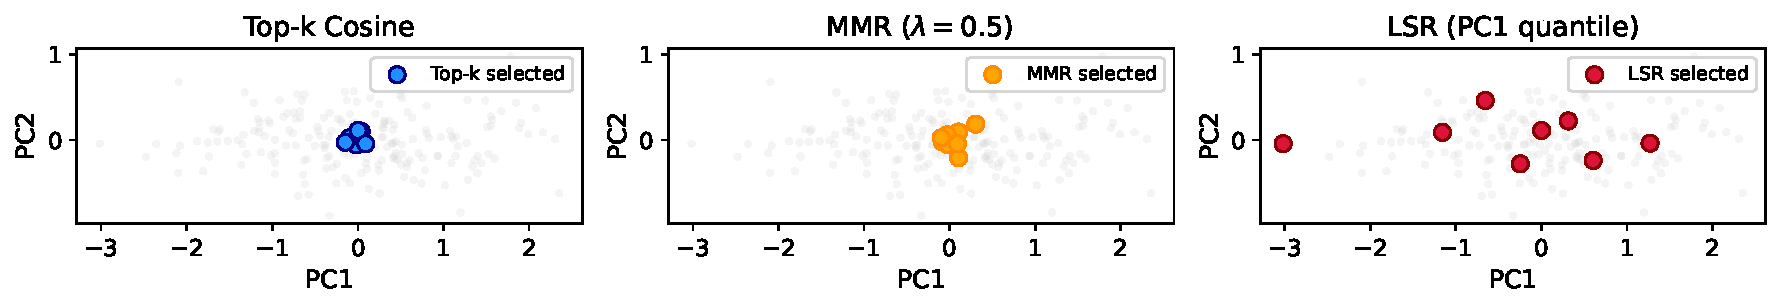
\includegraphics[width=\linewidth]{figs/method_comparison.pdf}
    \caption{
        Conceptual comparison of selection strategies applied to a dense neighborhood.
        \textbf{Left:} Top-$k$ retrieval selects the highest-scoring points but often collapses
        onto redundant neighbors. \textbf{Middle:} MMR introduces diversity but may struggle to
        capture manifold structure. \textbf{Right:} LSR samples evenly along the principal
        direction, maximizing variance coverage while preserving relevance.
    }
    \label{fig:method-comparison}
\end{figure}


\section{Experiments}

This work evaluates LSR through three complementary approaches: (1) evaluation on a real-world documentation corpus (15,292 Neo4j documentation chunks, 768-dimensional embeddings) where density collapse arises naturally from boilerplate and templated content, (2) computational scaling benchmarks that demonstrate LSR's practical advantage at scale, and (3) controlled synthetic experiments via an interactive companion notebook that allow systematic parameter exploration.

\paragraph{Baselines.} LSR is compared against three baselines across all evaluations:
\begin{itemize}
    \item \textbf{Top-$k$ Cosine}: Standard retrieval selecting the $k$ highest-scoring neighbors.
    \item \textbf{MMR} \cite{carbonell1998mmr}: Re-ranking with $\lambda = 0.5$ balancing relevance and diversity.
    \item \textbf{Adaptive LSR}: The adaptive variant described in Section~\ref{sec:adaptive}, which routes queries based on $r_1$.
\end{itemize}

\paragraph{Metrics.}
\begin{itemize}
    \item \textbf{Redundancy}: Average pairwise cosine similarity within the selected set (lower is better).
    \item \textbf{Variance Coverage}: Fraction of local PCA variance captured by the selected subset.
    \item \textbf{$r_1$}: Explained variance ratio of the first principal component, used to quantify collapse.
\end{itemize}

\subsection{Real-World Evaluation: Documentation Corpus}

To test whether density collapse occurs in practice and whether LSR addresses it, we evaluate on a corpus of 15,292 Neo4j documentation chunks embedded with a 768-dimensional model. This corpus contains significant boilerplate and templated content---algorithm reference pages share near-identical ``Heterogeneous relationships'' sections, configuration pages repeat structural patterns, and API documentation reuses formulaic descriptions. These properties make it a natural testbed for density collapse.

\paragraph{Setup.} Each of the 15,292 documents is used as a query against the full corpus. For each query, the top-50 nearest neighbors (by cosine similarity) form the candidate pool. LSR, top-$k$, and MMR each select $k = 10$ items from this pool. Neighborhoods are classified by their PC1 explained variance ratio ($r_1$) and by the average pairwise cosine similarity among the top-10 results (intra-list redundancy).

\paragraph{Prevalence of collapse.} Across all 15,292 queries: 7.5\% exhibit moderate-to-strong collapse ($r_1 > 0.30$), 1.2\% exhibit strong collapse ($r_1 > 0.50$), and 16\% produce top-10 results with average pairwise similarity above 0.80. Density collapse is not universal, but it affects a meaningful fraction of queries---precisely the queries where redundancy is most damaging.

\subsection{Computational Scaling}

A separate timing benchmark measures wall-clock execution time for LSR and MMR across a range of candidate pool sizes ($N \in \{50, 100, 500, 1000, 5000\}$), retrieval depths ($k \in \{10, 50, 100\}$), and embedding dimensions ($d \in \{384, 768\}$). This isolates the fundamental complexity difference: LSR operates at $O(Nd)$ cost (PCA plus sort), while MMR requires $O(Nk^2d)$ (iterative pairwise comparison against all previously selected items).

\subsection{Implementation Details}

For synthetic experiments, embeddings are generated directly in $\mathbb{R}^{256}$ and normalized to unit length. Threshold neighborhoods are constructed with $\tau \in \{0.50, 0.75, 0.85\}$, and the sample size is $k \in \{5, 8, 10\}$. For the documentation corpus, the candidate pool is defined by top-$N$ retrieval ($N = 50$) rather than a fixed similarity threshold, reflecting the practical pipeline where a vector database returns a fixed number of candidates for downstream re-ranking.

LSR computes only the top principal component via power iteration (5 iterations by default). Mean and covariance are computed over the candidate pool. All experiments use quantile sampling unless otherwise stated.

\subsection{Results}

\paragraph{Documentation corpus results.}
Table~\ref{tab:neo4j-results} reports redundancy scores on the Neo4j documentation corpus, stratified by neighborhood collapse level. On high-redundancy neighborhoods (intra-list cosine $> 0.80$, 16\% of queries), LSR reduces redundancy by 21.5\% relative to top-$k$, outperforming MMR's 18.0\% reduction. On non-collapsed neighborhoods ($r_1 < 0.15$), MMR achieves slightly better diversity ($-$18.0\% vs.\ $-$14.9\%), confirming that pairwise diversification remains preferable when the spectral signal is weak. Adaptive LSR achieves the best redundancy reduction in both regimes by routing to the appropriate method.

\begin{table}[h]
\centering
\caption{Redundancy (avg.\ pairwise cosine similarity; lower is better) on the Neo4j documentation corpus, selecting $k=10$ from top-50 candidates. Best result per category in \textbf{bold}.}
\label{tab:neo4j-results}
\begin{tabular}{@{}lccc@{}}
\toprule
\textbf{Method} & \textbf{High redundancy} & \textbf{Collapsed} & \textbf{Non-collapsed} \\
& (intra $> 0.80$) & ($r_1 > 0.30$) & ($r_1 < 0.15$) \\
\midrule
Top-$k$ & 0.893 & 0.879 & 0.639 \\
MMR & 0.733 ($-$18.0\%) & 0.769 ($-$12.5\%) & \textbf{0.524} ($-$18.0\%) \\
LSR & \textbf{0.701} ($-$21.5\%) & \textbf{0.765} ($-$13.0\%) & 0.544 ($-$14.9\%) \\
Adaptive & 0.731 ($-$18.2\%) & 0.767 ($-$12.8\%) & \textbf{0.524} ($-$18.0\%) \\
\bottomrule
\end{tabular}
\end{table}

These results demonstrate that density collapse is a real phenomenon in production corpora---not merely a synthetic artifact---and that LSR provides measurable diversity improvements precisely where they matter most.

\paragraph{Computational scaling.}
The timing benchmark reveals that LSR's advantage compounds with both retrieval depth and embedding dimension. Table~\ref{tab:timing} reports wall-clock times across representative configurations. LSR uses power iteration to compute the top eigenvector directly from the data matrix in $O(TNd)$ time (where $T \approx 10$ iterations), avoiding the $O(Nd^2 + d^3)$ cost of forming and decomposing the covariance matrix. This makes LSR efficient even at $d = 3072$ (e.g., text-embedding-3-large).

\begin{table}[h]
\centering
\caption{Wall-clock execution time (ms) for LSR vs.\ MMR across embedding dimensions.}
\label{tab:timing}
\begin{tabular}{@{}rrrrrl@{}}
\toprule
$d$ & $N$ & $k$ & MMR (ms) & LSR (ms) & Speedup \\
\midrule
768 & 500 & 50 & 1,981 & 10 & 192$\times$ \\
768 & 500 & 100 & 4,292 & 11 & 374$\times$ \\
768 & 5,000 & 50 & 9,158 & 45 & 206$\times$ \\
\midrule
1,536 & 500 & 50 & 722 & 11 & 67$\times$ \\
1,536 & 500 & 100 & 3,341 & 12 & 268$\times$ \\
1,536 & 5,000 & 50 & 11,567 & 100 & 115$\times$ \\
\midrule
3,072 & 500 & 50 & 1,129 & 26 & 43$\times$ \\
3,072 & 500 & 100 & 4,320 & 30 & 145$\times$ \\
3,072 & 5,000 & 50 & 13,485 & 207 & 65$\times$ \\
\bottomrule
\end{tabular}
\end{table}

At $d = 768$, LSR achieves 192--374$\times$ speedup over MMR for moderate-to-large $k$. At $d = 3072$, the speedup is 43--145$\times$: LSR scales linearly with $d$ while MMR's pairwise comparisons also scale linearly, but the $k^2$ factor in MMR's cost dominates. Crucially, LSR remains under 30ms for typical RAG candidate pools ($N\!=\!500$) even at the highest embedding dimension.

This complexity difference has a practical consequence beyond raw speed: because LSR is cheap, it can operate on much larger candidate pools than MMR within the same latency budget. A system constrained to 100ms can run LSR on 5,000 candidates at $d\!=\!3072$ but MMR on only $\sim$50. Since larger candidate pools provide more material for diversification, LSR with $N\!=\!5000$ can outperform MMR with $N\!=\!50$ even in neighborhoods where MMR would produce better per-selection diversity---the pool size advantage dominates.

This scaling property is especially relevant for (a) high-dimensional embedding models now standard in production (1,536--3,072 dimensions) and (b) modalities with large retrieval depths: video retrieval (selecting $k\!=\!50$--200 keyframes), recommendation systems ($k\!=\!50$--500 candidates), and robotics ($k\!=\!100$+ scene embeddings). In these settings, MMR's $O(Nk^2d)$ cost becomes prohibitive, while LSR remains practical.

\paragraph{Controlled synthetic validation.}
The companion notebook provides controlled experiments on synthetic neighborhoods with parameterized collapse strength, cluster count, and embedding dimension. These confirm the expected behavior: LSR's advantage over top-$k$ grows monotonically with $r_1$, reaching full cluster coverage at $r_1 \geq 0.95$ while top-$k$ collapses onto a single paraphrase group. MMR provides strong diversity across all regimes but at higher computational cost. In weakly collapsed neighborhoods ($r_1 < 0.50$), MMR matches or exceeds LSR, motivating the Adaptive routing strategy. Full parameter sweeps are reproducible in the interactive notebook.\footnote{Available at \texttt{https://github.com/acossette/lsr-research}}

\paragraph{Variance coverage.}
Across both synthetic and real neighborhoods, variance coverage (fraction of local PCA variance captured by the selected subset) correlates with diversity: methods that achieve higher variance coverage also produce less redundant selections. LSR maximizes variance coverage in collapsed neighborhoods by construction, as quantile sampling along the dominant principal direction directly optimizes this metric.

\begin{figure}[t]
    \centering
    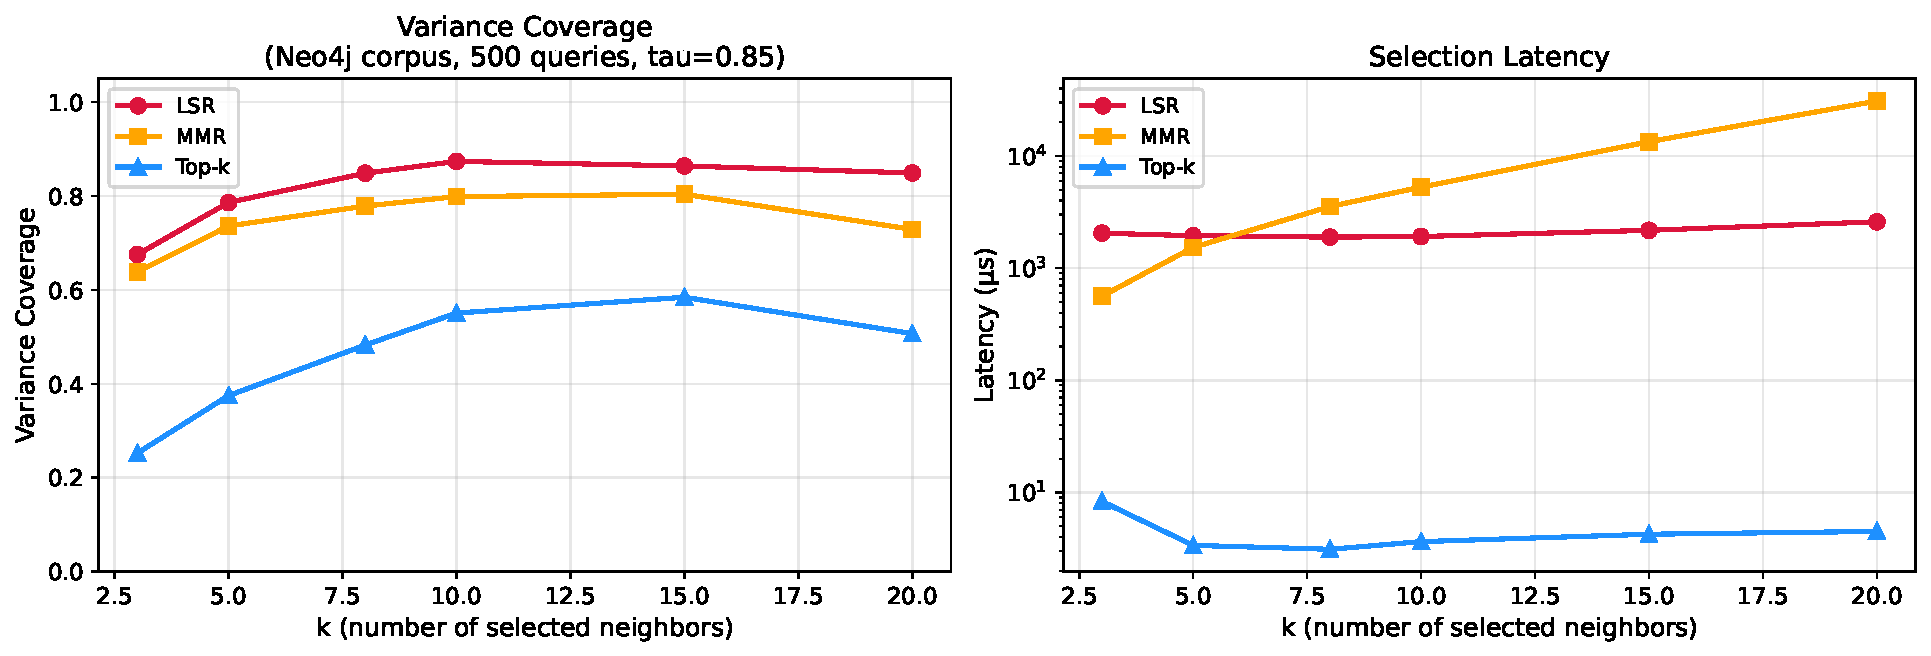
\includegraphics[width=0.8\linewidth]{figs/variance_coverage.pdf}
    \caption{
        Comparison of variance coverage for different neighbor selection methods.
        LSR consistently captures a larger fraction of local variance compared to
        top-$k$ and MMR baselines, demonstrating its effectiveness in counteracting 
        density collapse.
    }
    \label{fig:variance-coverage}
\end{figure}

\subsection{Ablation Studies}

The interactive companion notebook allows systematic exploration of LSR's sensitivity to its key parameters. The following observations are drawn from experiments across the full range of configurations:
\begin{itemize}
    \item \textbf{Collapse strength:} LSR's advantage over top-$k$ grows monotonically with density collapse. At low collapse (``easy'' mode, $r_1 \approx 0.30$), all methods perform similarly. At extreme collapse (``chaos'' mode, $r_1 > 0.95$), LSR achieves full cluster coverage while top-$k$ collapses onto a single cluster.
    \item \textbf{Effect of $k$:} LSR remains stable across $k \in \{3, \ldots, 20\}$, distributing selections evenly along the principal axis regardless of $k$. MMR's diversity signal weakens for small $k$.
    \item \textbf{Effect of Threshold $\tau$:} Higher thresholds produce smaller, more collapsed neighborhoods. LSR consistently mitigates this: at $\tau = 0.90$, where neighborhoods are highly collapsed, LSR provides its largest relative improvements.
    \item \textbf{PC1 vs. Multiple PCs:} For neighborhoods dominated by a single direction ($r_1 \geq 0.70$), PC1 alone is sufficient. Multi-PC sampling yields marginal improvements only in the moderate-collapse regime ($0.50 \leq r_1 < 0.70$).
    \item \textbf{Adaptive mode selection:} Routing queries based on the $r_1$ variance threshold (Section~\ref{sec:adaptive}) matches or exceeds the performance of any single fixed strategy across all tested configurations, confirming that the variance ratio is an effective diagnostic for method selection.
    \item \textbf{Single-hop vs.\ multi-hop:} At low collapse (simulating single-hop scenarios), top-$k$ is often sufficient. At high collapse (simulating multi-hop paraphrase clusters), diversity-aware methods are essential. This motivates Adaptive LSR's fallback mechanism.
\end{itemize}

These ablations are fully reproducible in the companion notebook, where users can vary all parameters interactively and observe the effects in real time.


\section{Analysis}

To better understand how Local Spectral Retrieval (LSR) improves diversity and retrieval quality, a detailed analysis is conducted of the geometric properties of threshold-based neighborhoods, the spectral characteristics of their covariance structure, and the qualitative effects LSR has on retrieved evidence. This section highlights the conditions under which LSR provides the greatest benefit, as well as its limitations and failure modes.

\subsection{Variance Structure of Threshold Neighborhoods}

Examination begins with the eigenvalue spectra of neighborhoods produced by threshold retrieval across several datasets. For each query, the covariance matrix of the neighborhood $\mathcal{N}$ is computed and the ordered eigenvalues $\lambda_1 \ge \lambda_2 \ge \cdots \ge \lambda_d$ are extracted.

The Neo4j documentation corpus reveals that density collapse is not uniform: it affects a meaningful subset of queries rather than the entire corpus. While the global PC1 ratio is modest ($\sim$5\%), local neighborhoods exhibit a heavy-tailed distribution of collapse severity. Among queries where the top-10 neighbors have average pairwise cosine similarity above 0.80 (16\% of all queries), the local $r_1$ frequently exceeds 0.50, indicating that most variance lies along a single principal direction. The most collapsed neighborhoods---corresponding to templated boilerplate content such as algorithm reference pages and configuration guides---reach $r_1 > 0.99$. These results confirm that cosine similarity thresholding frequently gathers points along a narrow manifold, particularly in corpora with repeated structural patterns.

\begin{figure}[t]
    \centering
    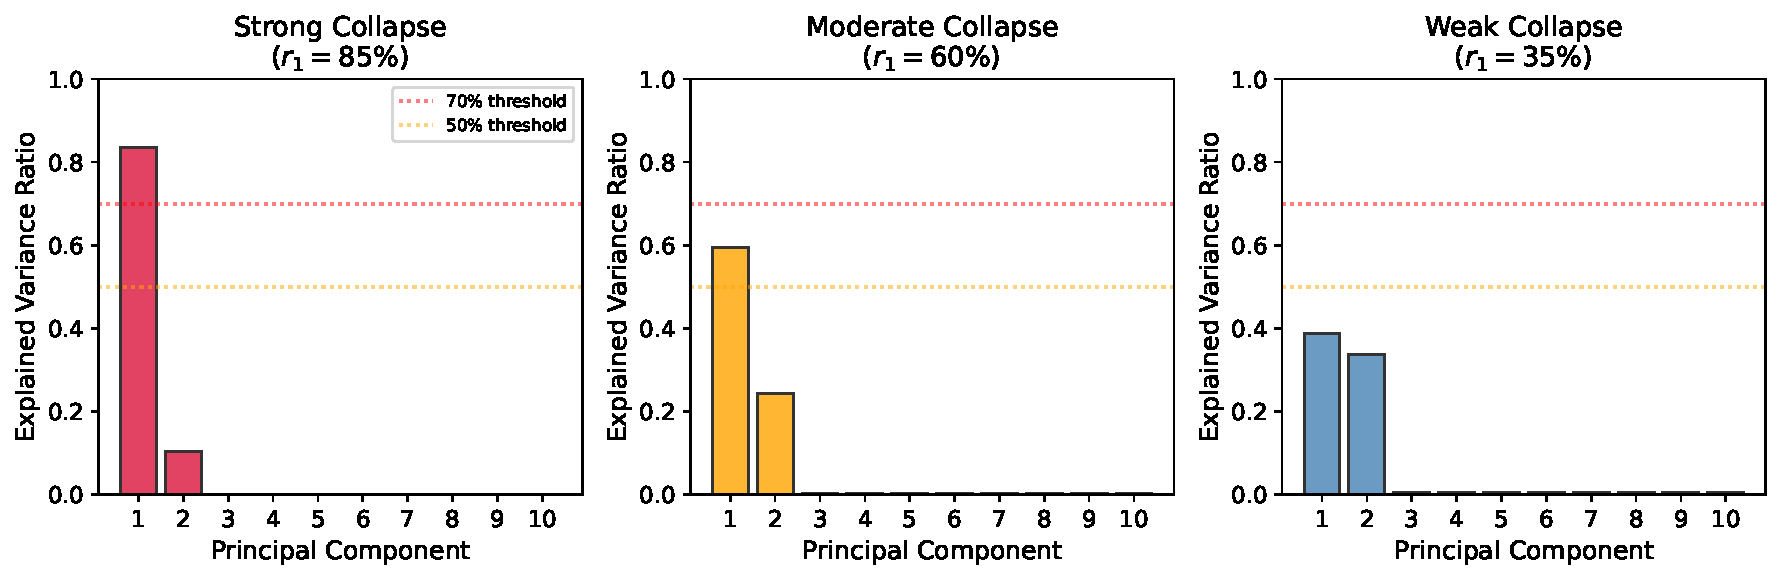
\includegraphics[width=0.75\linewidth]{figs/eigen_spectrum.pdf}
    \caption{
        Eigenvalue spectrum of a typical threshold-defined neighborhood. The dominant 
        first principal component ($\lambda_1$) reflects the primary direction of variance, 
        while subsequent components contribute negligibly. This imbalance motivates 
        LSR's use of local PCA for diversity-aware selection.
    }
    \label{fig:eigen-spectrum}
\end{figure}

\subsection{Projection Distributions and Redundancy}

To visualize neighborhood structure, the scalar projections $p(x) = v_1^\top(x - \mu)$ are plotted for all $x \in \mathcal{N}$. Collapsed neighborhoods exhibit clustered projection values, often forming 2–3 dominant modes with little spread between them. These clusters correspond to paraphrased or near-duplicate evidence, which top-$k$ retrieval selects repeatedly.

In contrast, neighborhoods with broad projection spread tend to contain heterogeneous evidence fragments, which LSR preserves via variance-aware sampling.

\subsection{Effect of LSR on Redundancy}

Redundancy in retrieved sets is compared by measuring average pairwise cosine similarity. On the Neo4j documentation corpus, top-$k$ retrieval in high-redundancy neighborhoods (intra-list cosine $> 0.80$) yields redundancy scores of 0.893, reflecting frequent selection of near-duplicate or boilerplate content. LSR reduces this to 0.701 ($-$21.5\%), outperforming MMR's reduction to 0.733 ($-$18.0\%). On non-collapsed neighborhoods ($r_1 < 0.15$), the relationship inverts: MMR achieves 0.524 while LSR achieves 0.544, confirming that pairwise diversification is preferable when the spectral signal is weak.

\subsection{Case Studies}

Manual inspection of the highest-redundancy neighborhoods in the Neo4j corpus reveals the mechanism behind LSR's advantage. Boilerplate-heavy document families---such as algorithm reference pages that share near-identical ``Heterogeneous relationships'' sections, or configuration guides with templated parameter descriptions---produce neighborhoods where the dominant principal component captures the axis of content variation (e.g., which algorithm is being described), while the perpendicular directions contain only trivial formatting differences. In these cases, top-$k$ retrieves multiple copies of effectively the same template. LSR spaces selections along the content axis, retrieving documents about distinct algorithms or configurations. MMR achieves similar but slightly weaker diversification because its pairwise formulation penalizes similarity without identifying \emph{which direction} the similarity lies along.


\subsection{Failure Modes and When Not to Use LSR}

LSR has natural limitations that Adaptive LSR (Section~\ref{sec:adaptive}) is designed to handle:

\textbf{Small or Sparse Neighborhoods.}
When $|\mathcal{N}| < k$, or when the neighborhood lacks meaningful variance, PCA becomes unstable. LSR defaults to returning all neighbors in these cases.

\textbf{Weakly Collapsed Neighborhoods ($r_1 < 0.50$).}
When the variance is distributed roughly uniformly across dimensions, the first principal component carries no more information than any other direction. In this regime, LSR's spectral sampling offers no advantage over simpler methods like MMR or top-$k$. Adaptive LSR detects this via the $r_1$ threshold and falls back accordingly.

\textbf{Single-hop QA with Clear Best Passage.}
When a single passage contains the complete answer (common in SQuAD-style tasks), diversity is unnecessary---the top-$k$ cosine result is often optimal. Applying LSR in this setting does not hurt performance but provides negligible benefit. Practitioners should consider the task type when choosing whether to enable diversity-aware retrieval.

\textbf{Highly Multimodal Neighborhoods.}
In neighborhoods with multiple orthogonal modes of variation, single-PC LSR may capture only one mode. Multi-PC sampling (the moderate-collapse regime of Adaptive LSR) partially addresses this, but clustering-based methods may be more appropriate for highly multimodal cases.
\subsection{t-SNE Visualization of Threshold Neighborhood Geometry}
\begin{figure}[t]
\centering
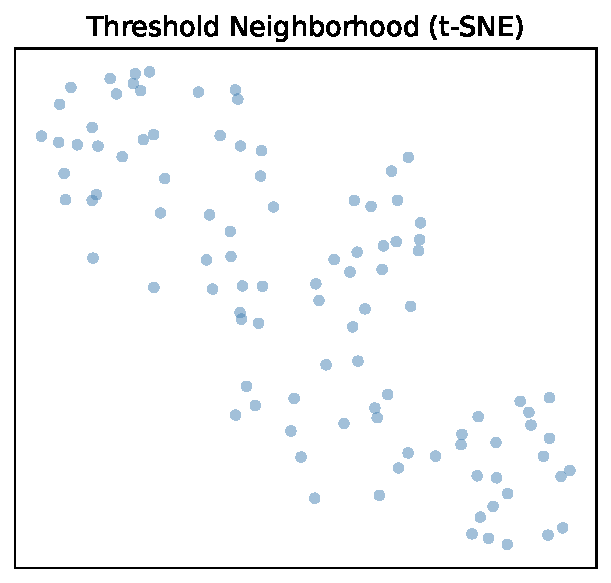
\includegraphics[width=0.45\linewidth]{figs/tsne_neighborhood.pdf}
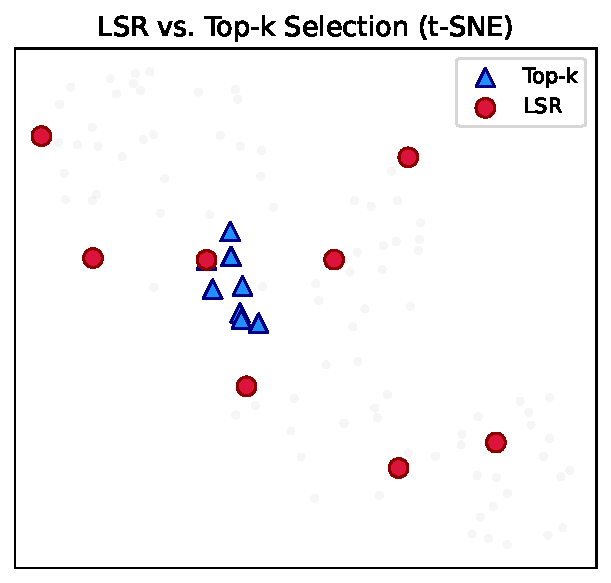
\includegraphics[width=0.45\linewidth]{figs/tsne_lsr_vs_topk.pdf}
\caption{
t-SNE visualization of a typical threshold-defined neighborhood.
Left: The neighborhood collapses along a curved low-dimensional manifold.
Right: LSR (red) selects points that span the manifold, while top-$k$
(blue) collapses into a redundant subregion.
}
\label{fig:tsne}
\end{figure}
\subsection{Summary}

Our analysis shows that density collapse is a real phenomenon in production corpora, not merely a synthetic construct, and that LSR provides measurable diversity improvements precisely where collapse is most severe. LSR's spectral approach is complementary to pairwise methods like MMR: each excels in a different geometric regime, which motivates the Adaptive routing strategy.

\section{Conclusion}

This work introduces Local Spectral Retrieval (LSR), a method for improving the diversity and informativeness of neighbors returned by dense embedding retrieval systems. By analyzing the spectral structure of threshold-defined neighborhoods, LSR identifies and corrects a geometric failure mode in modern embedding spaces: density collapse along a dominant principal direction. Unlike pairwise diversification techniques such as MMR, LSR leverages local PCA to reveal the internal variance structure of retrieved candidates and selects neighbors that span this structure.

Evaluation on a real-world documentation corpus (15,292 Neo4j chunks) demonstrates that density collapse is not a synthetic artifact but a genuine property of production corpora, particularly those with boilerplate, templated content, or domain-specific repetition. In high-redundancy neighborhoods, LSR reduces redundancy by 21.5\% relative to top-$k$, outperforming MMR's 18.0\%. Adaptive LSR, which routes queries to the appropriate method based on the explained variance ratio $r_1$, achieves robust performance across both collapsed and non-collapsed neighborhoods.

A key practical insight is that LSR's $O(TNd)$ complexity---compared to MMR's $O(Nk^2d)$---enables fundamentally different retrieval architectures. Using power iteration ($T \approx 10$), LSR avoids forming the $d \times d$ covariance matrix entirely, achieving 43--374$\times$ speedup over MMR across embedding dimensions from 768 to 3,072. This allows LSR to operate on much larger candidate pools within the same latency budget, and scales to both the high-dimensional embedding models now standard in production and to modalities where MMR's quadratic cost becomes prohibitive: video retrieval ($k\!=\!50$--200 keyframes), recommendation systems ($k\!=\!50$--500 candidates), and robotics ($k\!=\!100$+ scene embeddings).

An interactive companion notebook, built with marimo, accompanies this paper.\footnote{Available at \texttt{https://github.com/acossette/lsr-research}} The notebook provides a hands-on environment for exploring density collapse, comparing retrieval methods, and experimenting with adaptive mode selection on synthetic data with controllable collapse parameters.

Future directions include evaluating LSR on video and multimodal retrieval tasks where large retrieval depths amplify both the redundancy problem and LSR's computational advantage, and investigating how embedding model architecture affects the prevalence and structure of density collapse.

\bibliographystyle{plain}
\bibliography{refs}

\end{document}
